\chapter{Design and Application}

\section{Project Initialization}

When setting up the project and its directory, Vite and Django both did most of the hard work. Django would initialise all the main boilerplate code including the main script along with a set of testing code and the settings file itself. Vite generated all the JSX code along with the basic CSS which is significantly lighter than Create-React-App as discussed in section 2.9. Thanks to these two build pipeline tools, it made it easy to begin development and set up a git repository.

\section{Github Actions}

When setting up the custom user model in Django, there were a few issues encountered with the project structure that resulted in a deep dive into how the abstract model is implemented internally. This resulted in needing to keep a few of the declared fields within the default abstract user and then setting them to null. Doing this would also necessitate a custom user manager in order to create protections for the user serializer whenever a new user account is created. As the university implemented account system does not have a public API, there is a need to implement a unique account management system for the purpose of this demo to protect user data. This custom user manager can be seen in Figure \ref{fig:abstract_user_manager}.

\pagebreak
\begin{figure}[H]
\begin{minted}[mathescape, friendly]{python}
class CustomUserManager(BaseUserManager):
   def create_user(self, username, email, password=None):
       if not username:
           raise ValueError("User must have a username.")
       if not email:
           raise ValueError("User must have an email address.")

       user = self.model(username=username, email=self.normalize_email(email))

       user.set_password(password)
       user.save(using=self._db)
       return user
\end{minted}
\caption{Custom user manager implementing the serializable methods for inserting user data into the database}
\label{fig:abstract_user_manager}
\end{figure}

As shown in Figure \ref{fig:abstract_user_manager}, in order to initialise a new user model there are normalizers that need to be called to ensure that an email and username is valid before inserting that data into the database. Without these calls, it would be possible to post data to the backend that is invalid or even cause a potential SQL injection attack. This is where unit tests were written within the project in order to protect from future issues of Django having an invalid state creating migrations from conflicting models within the system of the default user class and the overwritten abstract user class. The unit tests written were to test both the creation event within Django and using the built in pytest support systems provided within the library. This was incredibly useful in the moment as, had a different back-end framework been chosen such as flask, there would not have been out of the box support as available with this choice instead as discussed in chapter 2.4. This can then all be automated using a small YAML configuration file for every time a git commit is made and pushed to Github for private code storage. These tests would run and ensure that the project did not have any conflicting design elements and ensure that Django can always boot and run migrations without any issues between code changes. This level of automation gives a strong confidence later in chapter 4.8 when the project is deployed to the wider web with less of a fear of crashes or issues.

\pagebreak
\begin{figure}[ht]
\centering
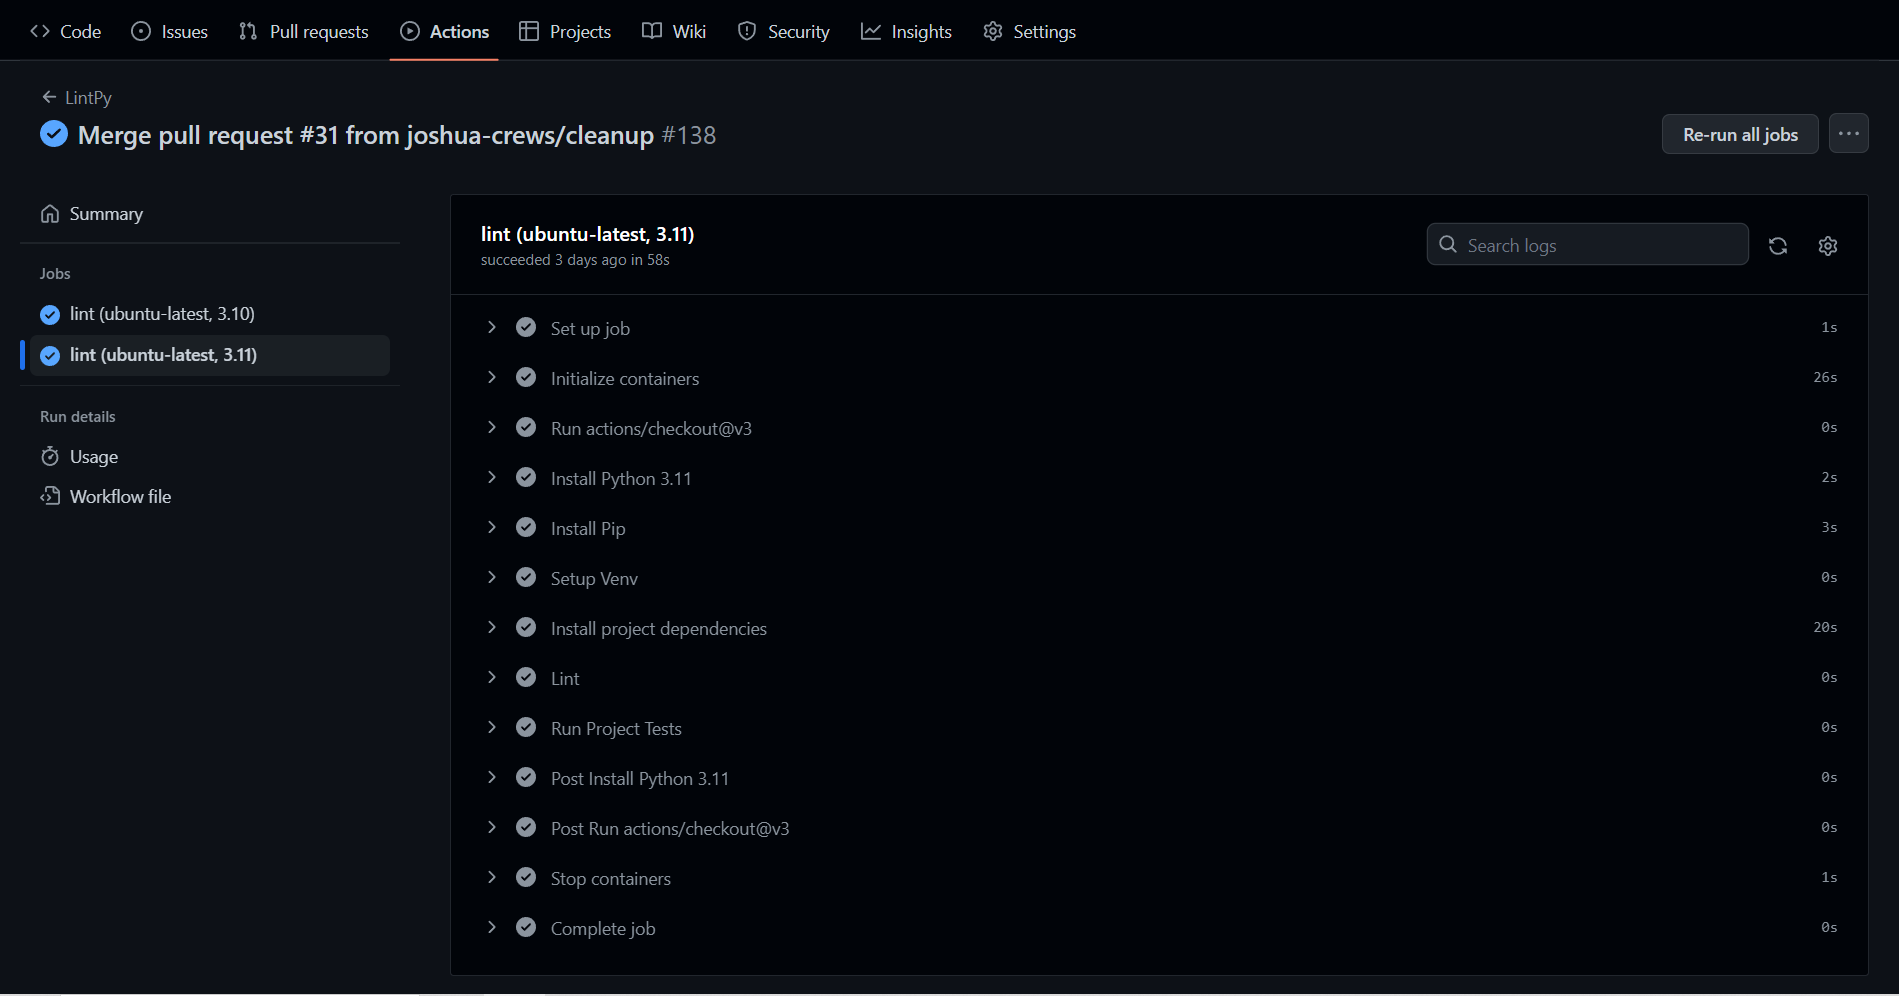
\includegraphics[width=15cm]{images/githubActions.png}
\caption{A sample actions running both a Flake8 lint configuration and project tests}
\label{fig:pipeline}
\end{figure}

When looking at Figure \ref{fig:pipeline}, it is nice to be able to see all the steps it automatically takes to configure a new docker container and run the project. This includes linting to ensure that both code quality is kept to a high standard but also to ensure that slowdowns are not implemented internally such as unused imports within python. Such issues are incredibly commonplace and the linter will catch all these issues and a failure if so, thus notifying the development team that there was an issue with the system. This includes the new user class as any changes would be caught quickly by the computer and can easily then be fixed with a new code commit.
\newline
\newline
The other advantage to having a pipeline is that it is easy to implement Github's dependabot to keep track of package updates and versioning of micropatches to used libraries. Having a test suite gives trust in our application and that any failures from an update would be caught and can be patched before upgrading versions. Any versions that pass the unit tests and can be assumed to be safely merged into the project and upgraded to the latest security patches without the fear of failure.

\section{Form HOC Component}

Moving to the front end of development, there were a couple of React features that were quite effective for development of the demo, including the usage of HOCs (Higher Order Components). A good example of this is the passing of what the user selected to the detailed form view. By using a higher order component, it is possible to pass in only the necessary hooks and data for the component to display the form data to the user. This makes it so that when the DOM is rendered to the client there is no extra data of all the fetched forms from the home page and instead the user’s client just has the one form displayed to them at the detailed form view. This also makes it so that any locator hook from the React Router package can be passed similar to dependency injection allowing the methods to be invoked to send the client to another location without compromising on calling the constructor a second time to create a new hook.
\newline
\newline
The only downside to using this method of HOCs is that all static methods have to be copied over or else the JavaScript JIT compiler will give a null pointer reference to undefined behaviour. This also means that all refs are not copied, but in this instance is not an issue as everything being used are objects rather than React refs.

\section{Form Validation}

The component on the front end that has by far the most complexity is the form page. Later in chapter 6 there will be discussion on improvements that could have been made and issues that arose during development of this part of the code. As demonstrated in section 2.8 and the design philosophy of Norman, obtaining information from the user in an easy to understand way is crucial for making a better user experience than that of the method provided by the university. One way to do this is to stage each input of information from the user in a logical set of questions with ample opportunity for the user to put in all the information about themselves.
\newline
\newline
The goal with staging each type of information input from the user is to provide a seamless experience of data validation without overwhelming the user as they read each question. As extenuating circumstance forms are filled in by a variety of users, some of whom may have serious medical complications or difficulties that lead to them needing to fill out a form in the first place, providing the best user experience is paramount to the frontend choices in design.
\newline
\newline
In order to implement a form system with a pagination system, a set of JSX divs were used and then hidden or shown given a current user index of where they were. This index would be incremented and then compared to the total number of present divs within the form. This also made it so that if a user clicks to add another module that was affected by their extenuating circumstance, it would simply add another div within the total amount. This makes it so that the user could never skip forward and submit an invalid form, but would also be prompted if they did not complete a field in its entirety. This would be a safeguard not present within the simple word document system the university currently uses and requiring double checking for all completed fields. 
\section{Django Endpoint Management}
As developing the backend would lead to many endpoints for management using a REST system, there was a need to have debugging tools at disposal. These tools would also need to be able to be turned off when deployed to a production environment so that potential threats could not exploit these weaknesses. The first set chosen was the response API provided by the Django Rest API. This provides a clear and interactable GUI for posting and fetching raw JSON data from the backend. Being able to do this through a localhost port rather than having to use the command line and CURL every time development is being done helps with simplicity and provides a clear set of reasons why something failed.
\newline
\newline
Another advantage of using the REST API is that it allows for easy use of the python debugger. Having the option of putting a breakpoint at an error is incredibly useful, especially when debugging the issues with the JWT management discussed in section 4.7.

\section{Database Structuring}

Django provides a library called Psycopg2 for interfacing with PostgresQL. As discussed in section 2.6, the advantages of SQL over the complications of configuring and setting up a document driven database are too great for the time frame of developing the demo. Psycopg2 however comes with a few caveats, with the first being that it is incredibly frustrating to install and set up on a UNIX machine. While development took place on a windows based machine and these issues were not fully realised at the time of development, there would later be permission issues with accessing the database user of postgres down the line when deployed to an AWS EC2 instance. The solution that was used was to pull the Psycopg2 binary and build from source on the local machine. While this took some time to understand and figure out how to do, it ultimately fixed the issue and would lead to being able to use the web application as normal.
\newline
\newline
When developing the database system itself, Django does provide a set of models. These models allow within native python code a declaration of a class and all the attributes about it. Each attribute is considered a field within the database, and Django provides an automatic migration function that will insert these fields into Postgres. This made it easy for configuring each field to exactly the information necessary to be stored, but also provided migration controls. These migration controls make it so that every time a new set of information needs to be inserted into the database, there would be protections of existing migrations as to not allow any collisions or nulls in non nullable fields. In the event such an instance would occur, Django would prompt the developer to create a one time entry for all these newly created columns to have and preserve previous entries from corruption.

\section{JWT Management}

In managing an account system, the back-end needs to have a set of endpoints for users to fetch and request JWT tokens. These tokens allow for getting other data at other endpoints such as their forms and creating a new form. The reason a token is needed is to protect user data and not require providing a password and username every time an endpoint is hit. To do this, when a user posts their username and password to get a new token, the back-end will then serve them an access token and a refresh token.
\newline
\newline
The access token is used for actions such as requesting forms or creating a new form, but expires every 10 minutes. This access token can also be used to encode account details such as if they are a faculty member or the student’s name. In the case of this demo, the token is actually used on the front end with some account details such as the student ID number to simplify filling in parts of the form and auto completion of certain fields. This makes it easier for the user as there is less information to fill out and they are not having to repeat actions.
\newline
\newline
In order to fetch a new access token, the client has a coroutine running in their browser to make a fetch for a new access token using their refresh token. The reason a refresh token is used for a new access token and not the old one is because should there ever be a compromise along the wire of the access token, the refresh token is only used for invalidating the old one. This means that if there is a breach in the middle of someone’s access token, their account is breached for a maximum of 10 minutes before the token expires. The refresh token makes it so that the user also does not have to log in every time they view the website, much like that of any large scale website today that users very rarely sign into.
\newline
\newline
The reason for using the JWT tokens is due to the simple to use library provided by the JWT python team but also as the added benefit that they can be stored within local storage of the browser. If CSRF tokens were used instead, this would require caching in the cookies of the browser which would require the user to accept the usage of cookies from the website which might be something they do not want. This makes JWT tokens not only the industry standard, but also the demo able to serve as many different non-technical users as possible.
\newline
\newline
One of the issues with issuing JWT tokens is that there is the possibility that you get an invalid fetch that can happen at times. This was found in development to be if too many tokens were requested and it happens concurrently, resulting in all tokens being blacklisted. This would ultimately cause a client to get signed out and have to sign back in so that a new refresh token can be obtained. While there is no immediate solution, there simply wasn’t an issue found in testing that resulted in needing to worry about this potential flaw in implementation.

\section{AWS Deployment for Survey}

In order to conduct the survey, participants are asked to use a deployed version of the demo, talk a little bit about their experience, and then compare that to the current implementation by the university for things they prefer about either. The goal of this survey is to understand what from the demo is absolutely critically loved and what would be needed first and foremost moving forward. In order to have participants use the demo however, a server would be needed to host and run the website along with the database for storing all credentials and blank information. To do this, a free AWS instance was used as it provided the minimum necessary computing power to host the instance as well as the option to open all necessary ports for network connectivity that would otherwise be impossible on a home network.
\newline
\newline
This AWS instance would also come packaged with Linux as its operating system, making it easy for setting up the project via git. As the source code of the project is kept private to the university, an access token for the server was issued for the duration of the project allowing it to fetch and update the code to sync with the master branch. Any changes to the master branch would then automatically alert the server and a reboot would be done to use the latest version. This made doing a day one patch discussed in section 5.1 much easier as all testing simply needed to be done on the local development machine and then merged with the master branch once ready.
\newline
\newline
Upon setting up the new instance, configuration of opening ports 22, 443, and 80 needed to be opened in order to allow for ssh, http, and https respectively. This would allow traffic to then make requests to the server and for Nginx to handle and direct that traffic to the correct WSGI server. This would either be for www traffic making a request to grab the front-end rendering of a page or the back-end routed to /api/ for convenience. Given the structure of the project, it was incredibly easy to then configure the front-end with a simple environment file where the back-end IP is hosted and how to hit each endpoint for fetching relevant information to a web page.
\newline
\newline
In order to further assist survey respondents with accessing the website, participants would need a somewhat memorable IP address rather than just a set of numbers to connect directly to the server. This would also provide some protection in case the instance ever went down and there would be a need for a server address change. To remedy these issues, a service called duckdns was chosen to provide a free IP along with their software for automatically updating the server address without users ever having to know. This made a memorable IP for users to connect to and traffic to be routed easily to all sub routes within the site.